\chapter{เวิร์กช็อปปัญญาประดิษฐ์การเรียนรู้เชิงลึกจำแนกโรคพืชและประเมินคุณภาพผลผลิตบนอุปกรณ์ฝังตัว}
\label{chap:ch12}

\section*{แผนบริหารการสอนประจำบทที่ 12}
\addcontentsline{toc}{section}{แผนบริหารการสอนประจำบทที่ 12}

\begin{planbox}{หัวข้อเนื้อหาประจำบท}
\begin{enumerate}[topsep=2pt, itemsep=1pt, partopsep=0pt, parsep=0pt, leftmargin=1.5em]
    \item รากฐานคอมพิวเตอร์วิทัศน์และพยาธิวิทยาพืชดิจิทัลในงานเกษตรแม่นยำ
    \item สถาปัตยกรรมการแบ่งชุดข้อมูลภาพถ่ายพืช 6 ชนิด 18 คลาส แบบรักษาสัดส่วน (Stratified Partitioning)
    \item โครงสร้างโครงข่ายประสาทเทียมแบบคอนโวลูชันขนาดกะทัดรัด (MobileNetV2, ResNet18 และ LeafNet)
    \item วิศวกรรมการฝึกสอนโมเดล การปรับแต่งอัตราการเรียนรู้แบบโคไซน์ และการหยุดการเรียนรู้ล่วงหน้า (Early Stopping)
    \item ระเบียบวิธีการประเมินผลเชิงลึก แผนภาพความสับสน (Confusion Matrix) และดัชนีชี้วัด F1-Score
    \item ปฏิบัติการควบคุมระบบผ่าน Leaf AI Studio Web Portal และการประมวลผลบน Google Colab GPU T4
    \item การส่งออกโมเดลสู่มาตรฐาน ONNX และ TorchScript สำหรับติดตั้งบนบอร์ดสมองกลฝังตัวภาคสนาม
    \item กรณีศึกษาการเชื่อมโยงระบบวินิจฉัยโรคพืชเข้ากับมาตรการฉีดพ่นสารชีวภัณฑ์อัตโนมัติ
\end{enumerate}
\end{planbox}

\begin{planbox}{วัตถุประสงค์เชิงพฤติกรรม}
\begin{enumerate}[topsep=2pt, itemsep=1pt, partopsep=0pt, parsep=0pt, leftmargin=1.5em]
    \item อธิบายหลักการแบ่งชุดข้อมูลแบบ Stratified Sampling และการทำงานของ Depthwise Separable Convolutions ได้อย่างถูกต้อง
    \item ออกแบบกระบวนการทำ Data Augmentation เพื่อลดปรากฏการณ์ Overfitting ในภาพถ่ายพืชได้อย่างเหมาะสม
    \item ดำเนินการฝึกสอนโมเดล Deep Learning ทั้งบนเครื่องคอมพิวเตอร์เฉพาะที่ (MPS GPU) และบนคลาวด์ Google Colab ได้อย่างคล่องแคล่ว
    \item วิเคราะห์ประสิทธิภาพโมเดลผ่าน Confusion Matrix และคำนวณค่า Precision, Recall และ F1-Score ได้อย่างแม่นยำ
    \item ส่งออกโมเดลโครงข่ายประสาทเทียมให้อยู่ในรูปไฟล์ ONNX และเขียนโปรแกรมอนุมานผล (Inference) บนบอร์ด Edge AI ได้อย่างสมบูรณ์
\end{enumerate}
\end{planbox}

\newpage

\begin{planbox}{วิธีสอนและกิจกรรมการเรียนการสอน}
\begin{enumerate}[topsep=2pt, itemsep=1pt, partopsep=0pt, parsep=0pt, leftmargin=1.5em]
    \item บรรยายเชิงทฤษฎีเปรียบเทียบสถาปัตยกรรม CNN ขนาดใหญ่กับโครงข่ายประสาทเทียมสำหรับอุปกรณ์ขอบเขต
    \item ปฏิบัติการสำรวจและแบ่งสัดส่วนชุดข้อมูลภาพถ่ายใบพืช 5,846 ภาพ ผ่านระบบ Leaf AI Studio
    \item ปฏิบัติการฝึกสอนโมเดลจริงบนคลาวด์ความเร็วสูง Google Colab ร่วมกับชิปเร่งความเร็ว Tesla T4 GPU
    \item ปฏิบัติการวิเคราะห์ผลการวินิจฉัยโรคและอ่านค่าแผนภาพความสับสนเพื่อค้นหาจุดอ่อนของโมเดล
    \item ปฏิบัติการทดสอบทำนายภาพใบพืชแบบสด (Inference Playground) และส่งออกไฟล์ ONNX สู่บอร์ดจริง
\end{enumerate}
\end{planbox}

\begin{planbox}{สื่อการเรียนการสอน}
\begin{enumerate}[topsep=2pt, itemsep=1pt, partopsep=0pt, parsep=0pt, leftmargin=1.5em]
    \item เว็บแอปพลิเคชันพอร์ทัล Leaf AI Studio ประจำโครงการ CMU AIoT 2027
    \item สมุดบันทึก Google Colab สำหรับฝึกสอนโมเดลด้วย GPU Tesla T4
    \item ชุดข้อมูลภาพถ่ายโรคพืชและคุณภาพผลผลิต 6 ชนิด 18 คลาส จำนวน 5,846 ไฟล์
    \item คอมพิวเตอร์ประมวลผลหรือบอร์ดสมองกลฝังตัว Raspberry Pi / บอร์ดไมโครคอนโทรลเลอร์ ESP32-CAM
    \item สไลด์ประกอบการสอนและคลังซอร์สโค้ดบน GitHub โครงการ aiot-workshop
\end{enumerate}
\end{planbox}

\begin{planbox}{การวัดและประเมินผล}
\begin{enumerate}[topsep=2pt, itemsep=1pt, partopsep=0pt, parsep=0pt, leftmargin=1.5em]
    \item การประเมินความถูกต้องในการแบ่งชุดข้อมูล Train, Validation และ Test ให้สมดุล
    \item ประสิทธิภาพของโมเดลที่ผ่านการฝึกสอน โดยพิจารณาจากค่าความแม่นยำและค่า Macro F1-Score
    \item ความสามารถในการแปลผลแผนภาพความสับสนและอธิบายสาเหตุความผิดพลาดของโมเดล
    \item ผลสำเร็จในการส่งออกโมเดล ONNX และการรันอนุมานผลภาพถ่ายใบพืชจริงได้อย่างถูกต้อง
\end{enumerate}
\end{planbox}

\newpage

\section{รากฐานคอมพิวเตอร์วิทัศน์และพยาธิวิทยาพืชดิจิทัลในงานเกษตรแม่นยำ}

การบริหารจัดการฟาร์มอัจฉริยะยุคใหม่จำเป็นต้องอาศัยการตรวจติดตามสุขภาพพืชอย่างต่อเนื่องและทันท่วงที โดยเฉพาะอย่างยิ่งอาการผิดปกติทางสรีรวิทยาและโรคพืชที่แสดงออกผ่านรอยโรคบนใบ (Leaf Lesions) ในอดีต เกษตรกรต้องอาศัยสายตาและความเชี่ยวชาญส่วนบุคคลในการเดินสำรวจแปลง ซึ่งมีข้อจำกัดอย่างยิ่งในด้านความครอบคลุม ความล่าช้า และความผิดพลาดจากการประเมินเชิงอัตวิสัย

การบูรณาการเทคโนโลยีคอมพิวเตอร์วิทัศน์ (Computer Vision) เข้ากับโครงข่ายประสาทเทียมแบบสังเคราะห์ (Convolutional Neural Networks หรือ CNN) ช่วยให้ระบบตรวจวัดอัตโนมัติสามารถคัดกรองอาการโรคได้อย่างรวดเร็วในระดับเสี้ยววินาที ดังแสดงความสัมพันธ์ในการคำนวณคอนโวลูชัน 2 มิติระหว่างภาพนำเข้า $I$ และเคอร์เนลตัวกรอง $K$ ขนาด $k \times k$ ตามสมการ

\begin{equation}
    S(i, j) = (I * K)(i, j) = \sum_{m=-p}^{p} \sum_{n=-p}^{p} I(i-m, j-n) K(m, n)
\end{equation}

\noindent โดยที่ $p = \lfloor k/2 \rfloor$ คือรัศมีของเคอร์เนล ค่า $S(i, j)$ แสดงถึงแผนที่ลักษณะเด่น (Feature Map) ที่ดึงคุณลักษณะเฉพาะของรอยโรค เช่น ขอบแผล ขอบใบไหม้ จุดสีสนิม และลวดลายเส้นใบ เพื่อส่งต่อไปยังชั้นจำแนกประเภท

\begin{figure}[H]
    \centering
    \resizebox{0.88\textwidth}{!}{
    \begin{tikzpicture}[node distance=1.8cm, auto, >=stealth]
        \tikzstyle{block} = [rectangle, draw=rbruNavy, fill=rbruNavy!8, text width=2.8cm, text centered, rounded corners, minimum height=1.2cm, font=\small\bfseries]
        \tikzstyle{line} = [draw=rbruNavy, thick, ->]
        
        \node [block] (input) {ภาพใบพืชนำเข้า\\(224$\times$224 RGB)};
        \node [block, right of=input, node distance=3.6cm] (conv) {Feature Extraction\\(MobileNetV2 / CNN)};
        \node [block, right of=conv, node distance=3.6cm] (pool) {Global Average Pooling};
        \node [block, right of=pool, node distance=3.6cm] (dense) {Dense Classifier\\(Softmax 18 Classes)};
        
        \path [line] (input) -- (conv);
        \path [line] (conv) -- (pool);
        \path [line] (pool) -- (dense);
    \end{tikzpicture}
    }
    \caption{แผนผังการไหลของข้อมูลในโครงข่ายประสาทเทียมเพื่อจำแนกโรคพืชและคุณภาพผลผลิต}
    \label{fig:cnn_pipeline}
\end{figure}

\section{ชุดข้อมูลภาพถ่ายพืช 6 ชนิดและการแบ่งสัดส่วนแบบรักษาสัดส่วน}

ชุดข้อมูลที่ใช้ในเวิร์กช็อปนี้ ประกอบด้วยภาพถ่ายจริงของใบพืชและผลผลิตทางการเกษตร 6 ชนิด รวมทั้งสิ้น 5,846 ภาพ ครอบคลุม 18 คลาสโรคและคุณภาพผลผลิต ได้แก่ ข้าวโพด (Corn), มันฝรั่ง (Potato), ส้ม (Orange), มะม่วง (Mango), กล้วย (Banana) และกาแฟ (Coffee)

ในงานจำแนกประเภทภาพทางการเกษตร ปัญหาสำคัญที่มักพบคือความไม่สมดุลของจำนวนตัวอย่างในแต่ละคลาส (Class Imbalance) หากใช้การสุ่มแบบปกติ (Uniform Random Split) คลาสที่มีจำนวนภาพน้อยอาจไม่ปรากฏในชุดทดสอบหรือชุดตรวจสอบเลย ส่งผลให้โมเดลไม่สามารถเรียนรู้ลักษณะเฉพาะของโรคนั้นได้ ด้วยเหตุนี้ ระบบจึงใช้ระเบียบวิธีแบ่งแบบรักษาสัดส่วน (Stratified Partitioning) เพื่อรักษาอัตราส่วนตัวอย่างของทุกคลาสให้เท่าเทียมกันในทุกชุดข้อมูล ดังแสดงในตารางที่ \ref{tab:dataset_distribution}

\captionsetup[table]{position=top, skip=6pt, labelfont={bf,color=rbruNavy}, textfont={normalfont}, labelsep=thaisep, justification=raggedleft, singlelinecheck=false}
\begin{table}[H]
    \caption{การกระจายตัวของชุดข้อมูลภาพถ่ายพืช 6 ชนิด 18 คลาส ตามสัดส่วน Stratified 70 : 15 : 15}
    \label{tab:dataset_distribution}
    \centering
    \begin{tabularx}{\textwidth}{p{3.0cm}YYYYR}
        \toprule
        \textbf{ชนิดพืชเป้าหมาย} & \textbf{จำนวนคลาส} & \textbf{Train (70\%)} & \textbf{Val (15\%)} & \textbf{Test (15\%)} & \textbf{รวมภาพทั้งหมด} \\
        \midrule
        ข้าวโพด (Corn) & 4 คลาส & 2,746 & 589 & 589 & 3,924 ภาพ \\
        มันฝรั่ง (Potato) & 3 คลาส & 630 & 135 & 136 & 901 ภาพ \\
        ส้ม (Orange) & 2 คลาส & 298 & 64 & 64 & 426 ภาพ \\
        มะม่วง (Mango) & 3 คลาส & 168 & 36 & 36 & 240 ภาพ \\
        กล้วย (Banana) & 3 คลาส & 143 & 31 & 31 & 205 ภาพ \\
        กาแฟ (Coffee) & 3 คลาส & 105 & 22 & 23 & 150 ภาพ \\
        \midrule
        \textbf{รวมทั้งสิ้น (All)} & \textbf{18 คลาส} & \textbf{4,092} & \textbf{877} & \textbf{877} & \textbf{5,846 ภาพ} \\
        \bottomrule
    \end{tabularx}
\end{table}

\section{สถาปัตยกรรมโครงข่ายประสาทเทียมสำหรับเอดจ์เอไอ}

ในการเลือกโครงสร้างโมเดลเพื่อนำไปติดตั้งบนอุปกรณ์ฝังตัว เช่น กล้องตรวจสภาพแปลง ESP32-CAM หรือคอมพิวเตอร์บอร์ดเดี่ยว Raspberry Pi มีข้อจำกัดด้านหน่วยความจำ (RAM/PSRAM) และกำลังประมวลผล ในเวิร์กช็อปนี้จึงออกแบบและรองรับ 3 สถาปัตยกรรมหลัก

\subsection{สถาปัตยกรรม MobileNetV2}
MobileNetV2 นำเสนอแนวคิดคอนโวลูชันแบบแยกส่วนลึก (Depthwise Separable Convolutions) ควบคู่กับบล็อก Inverted Residuals ที่มี Linear Bottlenecks ช่วยลดภาระการคำนวณ (FLOPs) และขนาดพารามิเตอร์ลงอย่างมหาศาล โดยมีอัตราส่วนการลดทอนภาระการคำนวณเมื่อเทียบกับคอนโวลูชันมาตรฐาน ตามสมการ

\begin{equation}
    \text{Reduction Ratio} = \frac{D_K \cdot D_K \cdot M \cdot D_F \cdot D_F + M \cdot N \cdot D_F \cdot D_F}{D_K \cdot D_K \cdot M \cdot N \cdot D_F \cdot D_F} = \frac{1}{N} + \frac{1}{D_K^2}
\end{equation}

\noindent โดยที่ $D_K$ คือขนาดของเคอร์เนลตัวกรอง (เช่น $3 \times 3$), $D_F$ คือมิติของแผนที่ลักษณะเด่น, $M$ คือจำนวนช่องสัญญาณนำเข้า และ $N$ คือจำนวนช่องสัญญาณส่งออก หากกำหนด $D_K = 3$ การคำนวณจะลดลงประมาณ 8 ถึง 9 เท่าเมื่อเทียบกับโครงข่ายดั้งเดิม

\subsection{สถาปัตยกรรม LeafNet}
เพื่อรองรับบอร์ดไมโครคอนโทรลเลอร์ขนาดเล็ก เช่น ESP32-S3 ทีมวิจัยได้พัฒนาโครงสร้างเฉพาะชื่อ \textbf{LeafNet} ประกอบด้วยบล็อกคอนโวลูชัน 4 ลำดับขั้นที่เชื่อมต่อด้วย Batch Normalization และ Leaky ReLU ฟังก์ชัน มีขนาดพารามิเตอร์รวมเพียง 1.2 ล้านพารามิเตอร์ (ขนาดไฟล์น้ำหนักประมาณ 4.8 เมกะไบต์) ทำให้สามารถจัดเก็บในหน่วยความจำแฟลชและรันผ่าน PSRAM ของบอร์ดได้อย่างราบรื่น

\section{วิศวกรรมการฝึกสอนโมเดลและการหยุดการเรียนรู้ล่วงหน้า}

ฟังก์ชันการสูญเสียที่ใช้ในการฝึกสอนคือ Cross-Entropy Loss ร่วมกับกลไก Label Smoothing เพื่อป้องกันไม่ให้โมเดลมีความมั่นใจเกินจริง (Overconfidence) ในคลาสใดคลาสหนึ่ง ตามสมการ

\begin{equation}
    \mathcal{L}_{\text{CE}} = -\sum_{c=1}^{C} y_{c}^{\text{smooth}} \log(\hat{y}_c)
\end{equation}

\noindent โดยที่ $\hat{y}_c = \frac{e^{z_c}}{\sum_{j=1}^C e^{z_j}}$ คือค่าความน่าจะเป็นที่ได้จากฟังก์ชัน Softmax และ $y_c^{\text{smooth}} = (1 - \epsilon) y_c + \frac{\epsilon}{C}$ เมื่อ $\epsilon = 0.1$ คือพารามิเตอร์การเกลี่ยค่าความน่าจะเป็น

การปรับอัตราการเรียนรู้ (Learning Rate Schedule) เลือกใช้แบบ Cosine Annealing ซึ่งจะค่อยๆ ปรับลดค่าอัตราการเรียนรู้จากค่าเริ่มต้น $\eta_{\text{max}} = 0.001$ ลงสู่ $\eta_{\text{min}} = 10^{-6}$ ตามสมการ

\begin{equation}
    \eta_t = \eta_{\text{min}} + \frac{1}{2}(\eta_{\text{max}} - \eta_{\text{min}})\left(1 + \cos\left(\frac{t}{T_{\text{max}}}\pi\right)\right)
\end{equation}

\noindent ควบคู่กับระบบ Early Stopping ที่จะยุติการฝึกสอนทันทีหากค่าความสูญเสียในชุดตรวจสอบ (Validation Loss) ไม่ดีขึ้นติดต่อกันเกิน 5 รอบ เพื่อป้องกันปัญหาการเรียนรู้เกิน (Overfitting) อย่างมีประสิทธิภาพ

\section{ระเบียบวิธีการประเมินผลเชิงลึกและแผนภาพความสับสน}

การประเมินประสิทธิภาพของระบบวิชันเอไอทางการเกษตร ไม่สามารถพิจารณาจากค่าความแม่นยำรวม (Overall Accuracy) เพียงอย่างเดียวได้ เนื่องจากความผิดพลาดในการตรวจไม่พบโรคที่มีความรุนแรง (False Negative) ย่อมก่อให้เกิดความเสียหายทางเศรษฐกิจแก่แปลงเกษตรมากกว่า การประเมินจึงอาศัยตัวชี้วัดความแม่นยำจำเพาะ (Precision), สภาพไว (Recall) และค่า $F_1$-Score ร่วมกับแผนภาพความสับสน (Confusion Matrix)

\begin{equation}
    \text{Precision} = \frac{TP}{TP + FP}, \quad \text{Recall} = \frac{TP}{TP + FN}
\end{equation}

\begin{equation}
    F_1 = 2 \cdot \frac{\text{Precision} \cdot \text{Recall}}{\text{Precision} + \text{Recall}}
\end{equation}

\noindent โดยที่ $TP$ คือตัวอย่างผลบวกจริง (True Positive), $FP$ คือผลบวกลวง (False Positive) และ $FN$ คือผลลบลวง (False Negative)

\begin{figure}[H]
    \centering
    \resizebox{0.65\textwidth}{!}{
    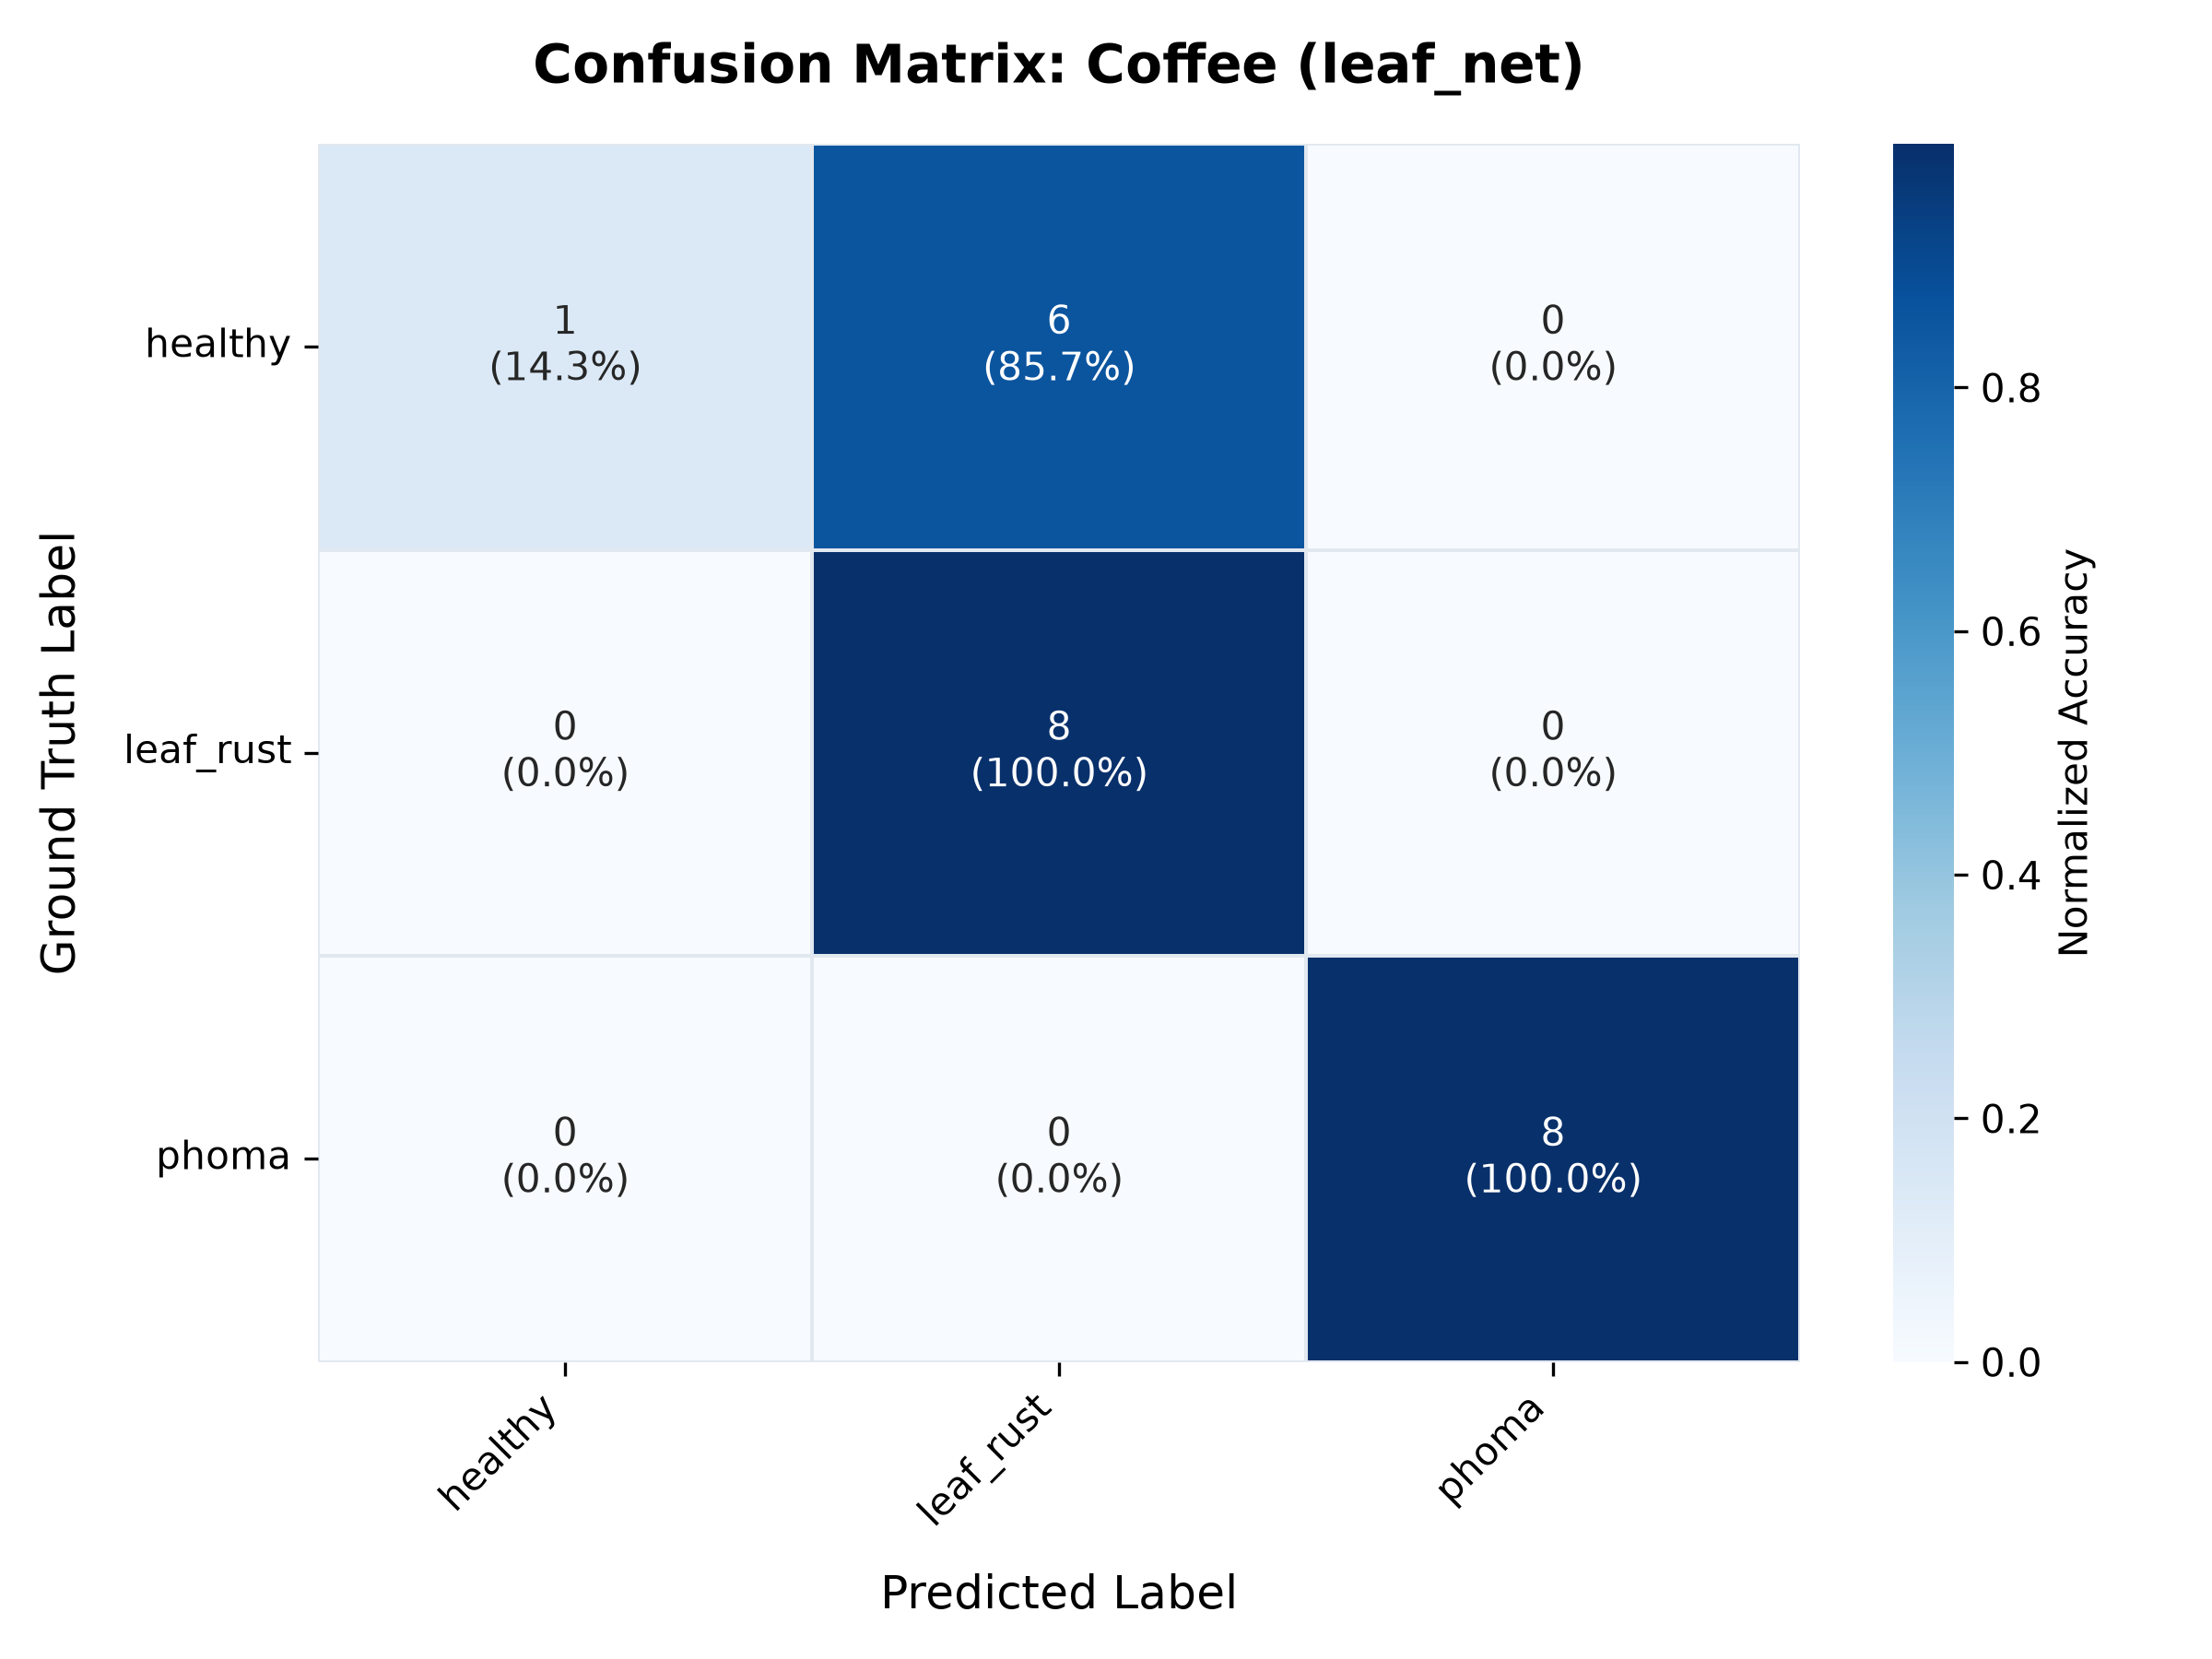
\includegraphics{figures/coffee_leaf_net_confusion_matrix.png}
    }
    \caption{แผนภาพความสับสน (Confusion Matrix Heatmap) แสดงผลการจำแนกโรคใบกาแฟ 3 คลาส}
    \label{fig:confusion_matrix}
\end{figure}

\section{ปฏิบัติการควบคุมระบบผ่าน Leaf AI Studio และ Google Colab}

ระบบ Leaf AI Studio ถูกออกแบบมาเพื่ออำนวยความสะดวกในการจัดอบรมเชิงปฏิบัติการ ผู้เรียนสามารถเข้าถึงหน้าต่างควบคุมผ่านเว็บเบราว์เซอร์ที่อยู่ ณ ที่อยู่ \url{http://localhost/cmu_aiot/leaf_ai_system/} โดยมี 6 ขั้นตอนหลักในการทดลอง

\begin{enumerate}
    \item \textbf{ขั้นตอนที่ 1 สำรวจและแบ่งชุดข้อมูล (Dataset Partitioning):} เลือกพืชเป้าหมาย กำหนดอัตราส่วนผ่านแถบเลื่อน และกดปุ่มเพื่อสร้างไฟล์ Manifest
    \item \textbf{ขั้นตอนที่ 2 เลือกสถาปัตยกรรมโมเดล (Model Selection):} เลือกระหว่าง MobileNetV2, ResNet18 หรือ LeafNet พร้อมกำหนดขนาดชุดข้อมูลย่อยและอัตราการเรียนรู้
    \item \textbf{ขั้นตอนที่ 3 สั่งฝึกสอนโมเดลสด (Live Training):} เลือกรันบนเครื่องคอมพิวเตอร์จริงผ่านการเร่งความเร็วฮาร์ดแวร์ หรือคลิกปุ่มเปิดรันบน Google Colab เพื่อใช้ GPU Tesla T4 ฟรี
    \item \textbf{ขั้นตอนที่ 4 ประเมินผลบนชุดทดสอบ (Model Evaluation):} วิเคราะห์ค่าสถิติ F1-Score และตรวจสอบจุดผิดพลาดผ่าน Heatmap
    \item \textbf{ขั้นตอนที่ 5 ห้องทดลองทำนายภาพสด (Inference Playground):} อัปโหลดภาพถ่ายใหม่หรือเลือกจากคลังตัวอย่าง เพื่อสังเกตผลการจำแนกและความเชื่อมั่น
    \item \textbf{ขั้นตอนที่ 6 การส่งออกโมเดล (Model Export):} ส่งออกโมเดลสู่รูปแบบ ONNX และ TorchScript เพื่อนำไปติดตั้งบนอุปกรณ์ภาคสนาม
\end{enumerate}

\section{การส่งออกโมเดลสู่มาตรฐาน ONNX และการติดตั้งบนอุปกรณ์สมองกลฝังตัว}

โมเดลที่ผ่านการฝึกสอนจะถูกบันทึกในรูปแบบ PyTorch Checkpoint (`.pth`) ซึ่งต้องพึ่งพาสภาพแวดล้อมภาษาไพธอนขนาดใหญ่ ในการนำไปใช้งานจริงบนบอร์ดสมองกลฝังตัว ระบบจะทำการแปลงโมเดลให้อยู่ในมาตรฐานเปิด \textbf{ONNX (Open Neural Network Exchange)} ซึ่งสามารถรันผ่าน ONNX Runtime บนชิปประมวลผล ARM ได้อย่างมีประสิทธิภาพ

\begin{lstlisting}[language=Python, caption={Python snippet for ONNX inference on Edge AI board}]
import onnxruntime as ort
import numpy as np
from PIL import Image

# 1. Load ONNX model on Raspberry Pi or Edge AI device
session = ort.InferenceSession("coffee_leaf_net_best.onnx")

# 2. Resize leaf image to 224x224 and normalize
img = Image.open("field_leaf.jpg").convert("RGB").resize((224, 224))
img_data = (np.array(img).astype(np.float32) / 255.0 - [0.485, 0.456, 0.406]) / [0.229, 0.224, 0.225]
input_tensor = np.transpose(img_data, (2, 0, 1))[np.newaxis, ...].astype(np.float32)

# 3. Run model inference and get predicted class
outputs = session.run(None, {"input": input_tensor})
predicted_class_id = int(np.argmax(outputs[0]))
print(f"Predicted Class ID: {predicted_class_id}")
\end{lstlisting}

\section{สรุปสารัตถะ แบบฝึกหัด และกรณีศึกษาเชิงวิพากษ์}

บทเรียนเชิงปฏิบัติการนี้ได้สาธิตการเปลี่ยนผ่านจากระบบเกษตรดั้งเดิมสู่เกษตรแม่นยำด้วยการประยุกต์ใช้คอมพิวเตอร์วิทัศน์และปัญญาประดิษฐ์ฝังตัว การแบ่งชุดข้อมูลแบบรักษาสัดส่วนช่วยรับประกันความสมดุลของการเรียนรู้ ในขณะที่สถาปัตยกรรมอย่าง MobileNetV2 และ LeafNet ช่วยทลายข้อจำกัดด้านทรัพยากรการคำนวณบนอุปกรณ์ริมขอบ การส่งออกโมเดลสู่มาตรฐาน ONNX จึงเป็นกุญแจสำคัญที่เชื่อมโยงงานวิจัยในห้องปฏิบัติการสู่แปลงเกษตรกรรมที่ใช้งานได้จริง

\begin{tcolorbox}[colback=white, colframe=rbruNavy, title={\textbf{คำถามทบทวนและกรณีศึกษาประจำบทที่ 12}}]
\begin{enumerate}
    \item จงอธิบายความแตกต่างระหว่างคอนโวลูชันมาตรฐานกับ Depthwise Separable Convolutions พร้อมทั้งคำนวณสัดส่วนการลดทอนการคำนวณเมื่อใช้เคอร์เนลขนาด $5 \times 5$
    \item ในการตรวจวินิจฉัยโรคราสนิมใบกาแฟ (Coffee Leaf Rust) หากโมเดลมีค่า Precision เท่ากับ 0.95 แต่มีค่า Recall เพียง 0.50 จะส่งผลกระทบต่อการระบาดของโรคในแปลงอย่างไร?
    \item จงออกแบบสถาปัตยกรรมระบบตรวจจับโรคใบไหม้ในแปลงข้าวโพดขนาด 50 ไร่ โดยบูรณาการกล้องติดโดรนสำรวจเข้ากับโมเดล LeafNet บนเกตเวย์ภาคพื้นดิน
\end{enumerate}
\end{tcolorbox}
